\section{Na型モンモリロナイトの水和エネルギーモデル}
\subsection{水分浴の化学ポテンシャル}
粘土含水系が温度$T$,相対湿度$r_H$の水蒸気に接しているとする.
水蒸気は粘土含水系に対して水分浴の役割を果たし,
その化学ポテンシャル$\mu_w$と$r_H$の関係は次のように表される\cite{Tombach}.
\begin{equation}
	\mu_w
	=
	\mu_w^{sat} +k_BT \log
	\left\{
		\frac{\phi(P_w)}{\phi(P^{sat}_w)}
		r_H
	\right\}
	\label{eqn:mu_rH}
\end{equation}
ただし,$k_B(=1.380649\times 10^{-23}$[J/K])はボルツマン定数を,
$P_w$と$P^{sat}_w$は,それぞれ,水分浴の蒸気圧と飽和蒸気圧を表す.
また,$\phi(P)$は蒸気圧$P$におけるフガシティー係数を,
$\mu_w^{sat}$は$P=P^{sat}_w$における水分浴の化学ポテンシャルを意味する.
ここでは,簡単のためフガシティー係数を1とし,式(\ref{eqn:mu_rH})を
\begin{equation}
	\mu_w
	=
	\mu_w^{sat} +k_BT \log
	\left(
		r_H
	\right)
	\label{eqn:mu_rH_simple}
\end{equation}
として用いる.いま,水分浴と平衡状態にある粘土含水系の化学ポンテンシャルを$\mu$とすれば, 
$\mu$は水分浴の化学ポテンシャルに一致する.すなわち
\begin{equation}
	\mu=\mu_{w}
	\label{eqn:equiv_mu}
\end{equation}
が成り立つ.
\subsection{粘土含水系の自由エネルギー}
粘土含水系の自由エネルギーを$G$とする.粘土含水系内の水分に関する化学ポテンシャル
$\mu$は,$G$を水分子数$N$で微分し,
\begin{equation}
	\mu=\frac{\partial G}{\partial N}
	\label{eqn:mu_GN}
\end{equation}
で与えられる.ここで,CG-MD系のもつ自由エネルギーを,
粗視化粒子間相互作用ポテンシャル$\left<\Psi_{LJ}\right>$と
層間水の水和に関する自由エネルギー$G_{hyd}$に分割し,
次のように表す.
\begin{equation}
	G=\left< \Psi_{LJ} \right> +G_{hyd}
	\label{eqn:Gtot}
\end{equation}
このように表現した自由エネルギー$G$に対し,平衡状態で式(\ref{eqn:equiv_mu})
が満足されるように$G_{hyd}$を与える.
そこで,式(\ref{eqn:mu_rH_simple})と(\ref{eqn:Gtot})を式(\ref{eqn:equiv_mu})
に代入すれば,
\begin{equation}
	\frac{\partial G}{\partial N}
	=
	\frac{\partial \left< \Psi_{LJ}\right>}{\partial N}
	+
	\frac{\partial G_{hyd}}{\partial N}
	=
	\mu_w^{sat} +k_BT \log
	\left(
		r_H
	\right)
	\label{eqn:equiv_rH}
\end{equation}
が得られる.以下,$G_{hyd}$を水和エネルギーと呼ぶ.
なお,CG-MD法における相互作用ポテンシャルは,非平衡状態でも定めることができる.
一方,式(\ref{eqn:equiv_rH})は平衡状態で成り立つ式である.この点の区別を
つけるために,
平衡状態における相互作用ポテンシャルを
$\Psi_{LJ}$でなく$\left< \Psi_{LJ}\right>$と表記している. \\
\hspace{\parindent}
CG-MD系の相互作用ポテンシャルは,Lenard-Jonesポテンシャル:
\begin{equation}
	U(\fat{x}_i,\fat{x}_j; \sigma) 
	= 4 \varepsilon 
	\left\{ 
	\left(\frac{\sigma}{r_{ij}}\right)^{12}
	-
	\left(\frac{\sigma}{r_{ij}}\right)^6
	\right\}, \ \ \left( r_{ij}=\left| \fat{x}_i-\fat{x}_j\right| \right)
	\label{eqn:LJ}
\end{equation}
を用いて,
\begin{equation}
	\Psi_{LJ}=\sum_{i<j} U(\fat{x}_i,\fat{x}_j; \sigma) 
	\label{eqn:def_PsiLJ}
\end{equation}
で与えられる.ただし,$\fat{x}_i$と$\fat{x}_j$は,それぞれ,第$i$および第$j$番目
の粗視化粒子位置を表し,
$\varepsilon$は
\begin{equation}
	\varepsilon=1.0\times 10^{-19}, \ \ [{\rm Nm}]
	\label{eqn:eps_of_LJ}
\end{equation}
である.ポテンシャル$U$の基準距離$\sigma$は,層間距離を制御する変数であるとともに,
粗視化粒子に水和した水分量としての意味をもつ.平衡状態における相互作用ポテンシャルは,
式(\ref{eqn:def_PsiLJ})の時間$t$における瞬間値$\Psi_{LJ}(t)$の平均:
\begin{equation}
	\left< \Psi_{LJ}\right>
	=
	\frac{1}{T_d}\int_{t_0}^{t_0+T_d} \Psi_{LJ}(t)dt
	\label{eqn:Psi_eq}
\end{equation}
で与えられる.ただし,式(\ref{eqn:Psi_eq})において$T_d$は十分に長く,
対象とする系は時刻$t_0$に依存しない平均値を与える状態にあることを
前提としている.\\
\hspace{\parindent}
$\left< \Psi_{LJ} \right>$や$G_{hyd}$は熱力学的なマクロ量であることから,
温度$T$,圧力$P$, 水分子数$N$を独立変数として表すことができる.
ここでは,温度$T$は一定として引数から省略し,$P$と$N$を用いて
\begin{equation}
	G(P,N)=\left< \Psi_{LJ} \right>(P,N) +G_{hyd}(P,N)
	\label{eqn:Gtot_PN}
\end{equation}
と書く.系の体積$V$と化学ポテンシャル$\mu$は,自由エネルギー$G$の微分で
次のように与えられる.
\begin{eqnarray}
	V &= & 
	\left( \frac{\partial G}{\partial P} \right)_N 
	=
	\left( \frac{\partial \left< \Psi_{LJ}\right>}{\partial P} \right)_N 
	+
	\left( \frac{\partial G_{hyd}}{\partial P} \right)_N 
	\label{eqn:G2V}
	\\
	\mu &= & \left( \frac{\partial G}{\partial N} \right)_P 
	=
	\left( \frac{\partial \left< \Psi_{LJ}\right>}{\partial N} \right)_P 
	+
	\left( \frac{\partial G_{hyd}}{\partial N} \right)_P 
	\label{eqn:G2mu}
\end{eqnarray}
ここで,力学的な量である$\left<\Psi_{LJ}\right>$は系の体積$V$と圧力$P$の関係を,
層間水に関する量である$G_{hyd}$は水分量$N$と化学ポテンシャル$\mu$の関係を,
それぞれ,定めるエネルギー成分となるよう$G$が分割されていることを要請する.
すなわち,式(\ref{eqn:Gtot_PN})は
\begin{eqnarray}
	\left( \frac{\partial \left< \Psi_{LJ}\right>}{\partial N} \right)_P=0, 
	& \Leftrightarrow & 
	\left< \Psi_{LJ}\right>(P,N) = \left< \Psi_{LJ}\right>(P) 
	\label{eqn:assuption1}
	\\ 
	\left( \frac{\partial G_{hyd}}{\partial P} \right)_N =0
	& \Leftrightarrow & 
	 G_{hyd}(P,N) = G_{hyd}(N) 
	\label{eqn:G2mu}
	\label{eqn:asumption2}
\end{eqnarray}
を満足するような自由エネルギーの分割であるとする.
%($\Psi_{LJ}$はパラメータ$\sigma$を通じて$N$に依存するが,
%$\left<\Psi_{LJ}\right>$をある種の平衡状態について$N$に依存
%しないようにすることは可能である).
このとき,式(\ref{eqn:mu_GN})は,式(\ref{eqn:G2mu})より
\begin{equation}
	\mu= \left( \frac{\partial G_{hyd}}{\partial N} \right)_P 
	=
	\frac{dG_{hyd}}{dN}
	\label{eqn:G2mu_2}
\end{equation}
となり,平衡条件(\ref{eqn:equiv_rH})を次のように表すことができる.
\begin{equation}
	\frac{d G_{hyd}}{d N}
	=
	\mu_w^{sat} +k_BT \log \left( r_H \right)
	\label{eqn:mu_hyd}
\end{equation}
\subsection{粉末X線回折試験で得られる相対湿度と水分子数の関係}
式(\ref{eqn:mu_hyd})の両辺を水分子数\(N\)で積分することができれば,
水和エネルギー\(G_{hyd}\)が定められる.しかしながら,
式(\ref{eqn:mu_hyd})の左辺は\(N\)に関する式である一方,
右辺は相対湿度\(r_H\)を通じて\(N\)に依存する形になっている.
従って,$N$を変数として積分を行うには,\(r_H\)と\(N\)の関係が必要になる.
含水した粉末状の粘土に対しては, X線回折試験で得られた回折ピークから粘土層間の距離\(h\)
が求められる\cite{Morodome},\cite{Yamada}.諸留,河村\cite{Morodome}は,
相対湿度と温度を制御した環境下で,モンモリロナイトのX線回折試験を行い,
相対湿度$r_H$と層間距離$h$の関係:
\begin{equation}
	h=h(r_H), \ \ (0 \leq r_H \leq 1)
	\label{eqn:hz_rh}
\end{equation}
を,相対湿度0$\% (r_H=0)$から100$\% (r_H=1)$の範囲で詳細に調べている.
図\ref{fig:fig1}-(a)は,文献\cite{Morodome}に示された結果のうち,
Na型モンモリロナイトに対する温度50\(^\circ\)Cでの相対湿度と層間距離の
関係を再現したものである.
これを式(\ref{eqn:hz_rh})として用いれば,環境の相対湿度と
粘土の層間距離を結びつけることができる.
%--------------------
\begin{figure}[h]
	\begin{center}
	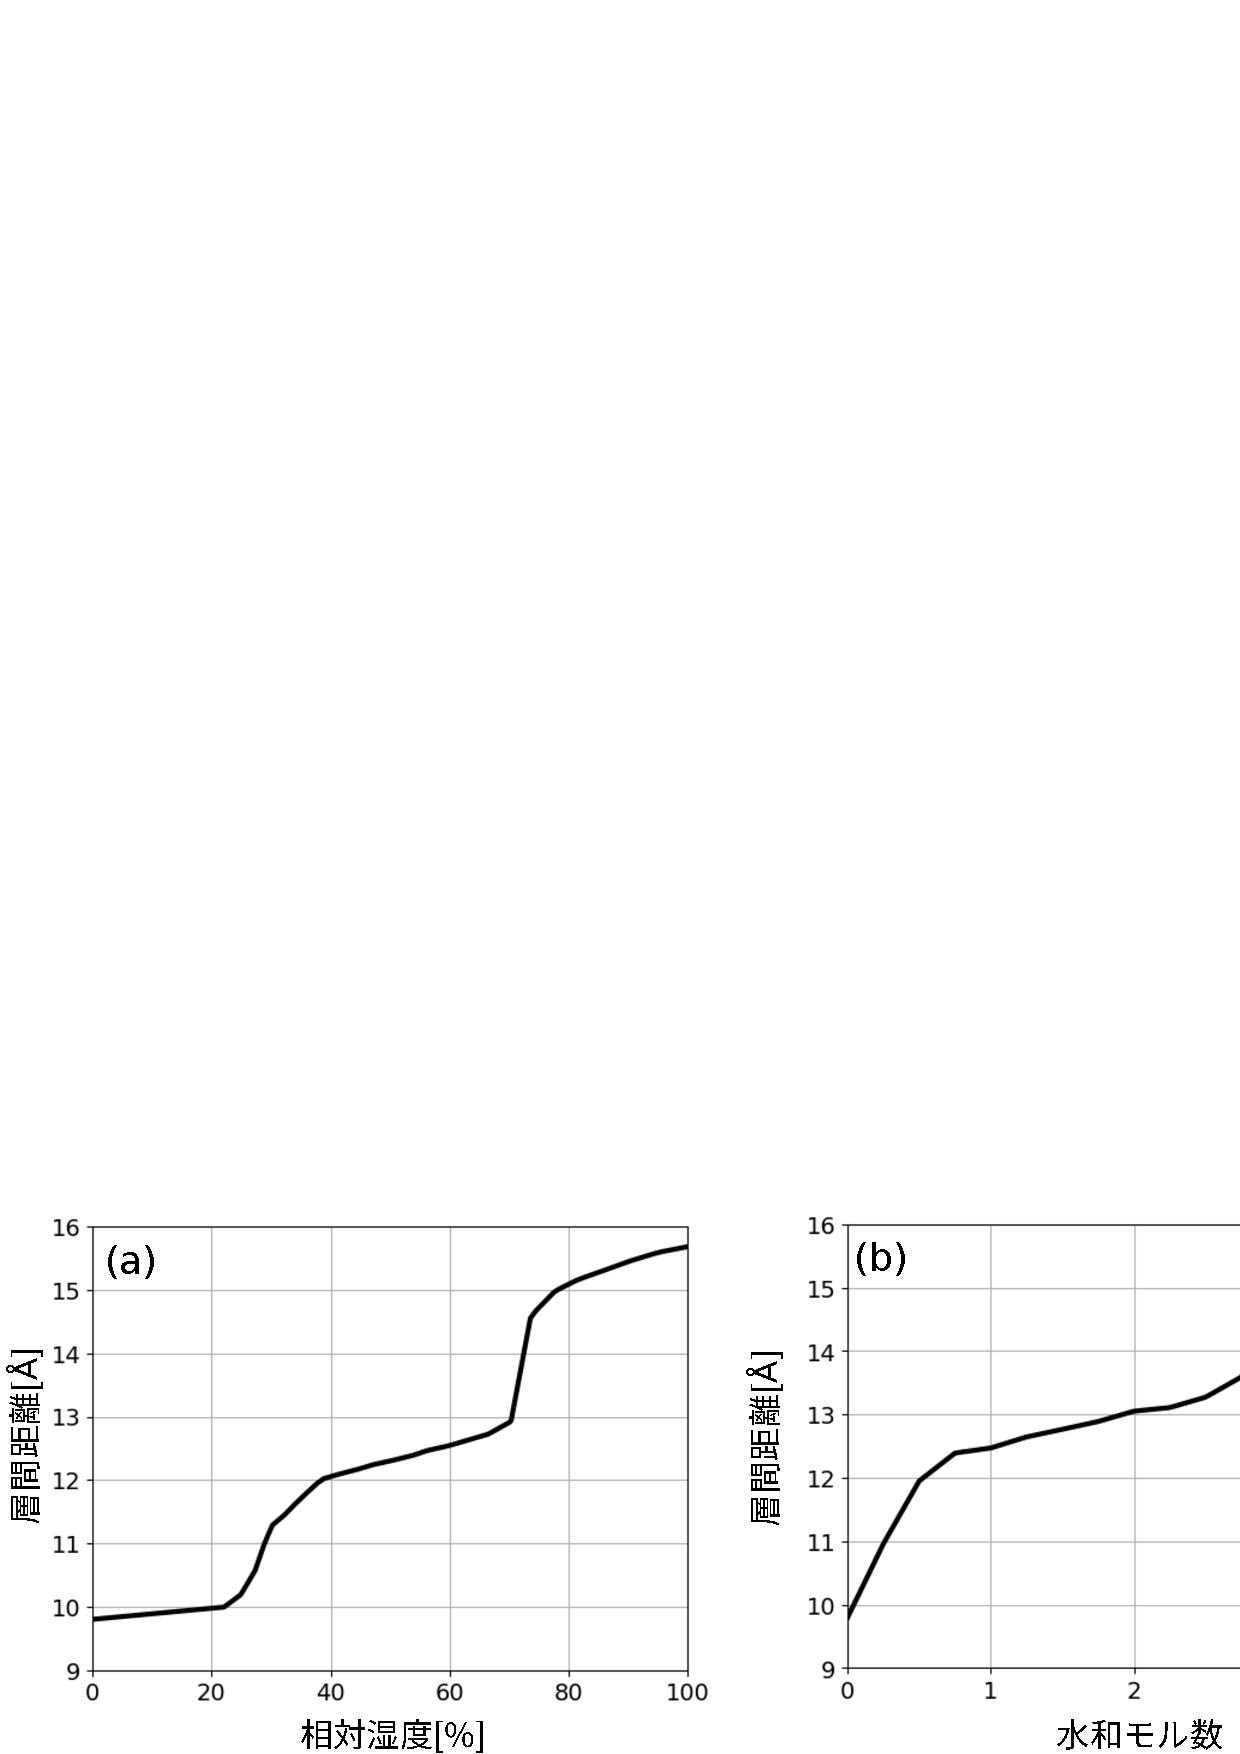
\includegraphics[width=1.0\linewidth]{Figs/fig1.pdf} 
	\end{center}
	\caption{
		Na型モンモリロナイトの膨潤挙動.
		(a)粉末X線回折試験で得られた相対湿度と層間距離の関係(諸留,河村\cite{Morodome}から再現).
		(b)全原子分子動力学計算で得れられた水和モル数と層間距離の関係(森本ら\cite{Morimoto}の
		データを使用). 
	} 
	\label{fig:fig1}
\end{figure}
これに加えて層間距離\(h\)と水分子数\(N\)の関係が得られば,
二つの関係をあわせて\(r_H\)と\(N\)の関係が定められる.
%式(\ref{eqn:mu_hyd})の両辺を\(N\)あるいは\(r_H\)に変数を統一して書くことができる.
そこで,層間距離$h$と水和モル数\(n\)の関係:
\begin{equation}
	h=h(n)
	\label{eqn:hz_nw}
\end{equation}
を全原子分子動力学計算で求める.
図\ref{fig:fig1}-(b)は,森本ら\cite{Morimoto}が行った全原子分子動力学計算の結果を,
$0\leq r_H \leq 1$で観測される層間距離範囲でプロットしたものである.
これら図\ref{fig:fig1}の結果を用い,式(\ref{eqn:hz_nw})と式(\ref{eqn:hz_rh})
を合成してその逆関数
\begin{equation}
	r_H=r_H(n)=r_H(h(n))
	\label{eqn:rh_nw}
\end{equation}
を数値的に求めると,図\ref{fig:fig6}が得られる.
%--------------------
\begin{figure}[h]
	\begin{center}
	\includegraphics[width=0.6\linewidth]{Figs/fig6.pdf} 
	\end{center}
	\caption{
		XRD測定結果\(h=h(r_H)\)と全原子分子動力学計算結果の\(h=h(n)\)
		から得られた,相対湿度$r_H$と水和モル数$n$の関係.
	} 
	\label{fig:fig6}
\end{figure}
%--------------------
式(\ref{eqn:mu_hyd})は任意の平衡状態で成り立つため,粉末X線回折試験
から得られた式(\ref{eqn:rh_nw})を用いれば,次項で示すように,水和エネルギー
を求めることができる.
\subsection{水和エネルギー}
式(\ref{eqn:rh_nw})を式(\ref{eqn:mu_hyd})に代入し,
\begin{equation}
	N=nN_A, \ \ (N_A=6.023\times 10^{23}:アボガドロ数)
	\label{eqn:}
\end{equation}
であることを考慮すれば,式(\ref{eqn:mu_hyd})の変数を\(n\)に統一した次の関係が得られる.
\begin{equation}
	\frac{d G_{hyd}}{d n}
	=
	\mu_w^{sat}N_A +k_BN_AT \log \left\{ r_H(n) \right\}
	\label{eqn:mu_hyd_n0}
\end{equation}
式(\ref{eqn:mu_hyd_n0})で,\(\mu_w^{sat}N_A\)は化学ポテンシャルを1molあたりの
エネルギーとして表したもので,\(k_B N_A\)は気体定数\(R\)に等しい.
そこで,これ以後,化学ポテンシャルの単位はJ/molであるとして,
式(\ref{eqn:mu_hyd_n0})から\(N_A\)を省略すれば,
\begin{equation}
	\frac{d G_{hyd}}{d n}
	=
	\mu_w^{sat} +RT \log \left\{ r_H(n) \right\}
	\label{eqn:mu_hyd_n}
\end{equation}
と書くことができる.ここで,式(\ref{eqn:mu_hyd_n})を温度一定のもと相対湿度$r_H=1$から
積分すれば,自由エネルギー変化:
\begin{equation}
	\Delta G_{hyd}(n) = G_{hyd}(n)-G_{hyd}(n_{sat})
	\label{eqn:del_G}
\end{equation}
が
\begin{equation}
	\Delta G_{hyd}(n)
	=
	\mu_{sat}\Delta n
	+
	RT
	\int_{n_{sat}}^{n} \log \left\{ r_H(n)\right\} dn, \ \ (0 \leq n \leq n_{sat})
	\label{eqn:del_G_mu}
\end{equation}
で計算できる. ただし,\(n_{sat}\)は相対湿度\(r_H=1\)のときに粉末状の粘土がもつ
層間水量を,\(\Delta n\)はその増分
\begin{equation}
	\Delta n = n-n_{sat}
\end{equation}
を意味する. また,粘土含水系の化学ポテンシャルは
\begin{equation}
	\mu(n)
	=
	\frac{d G}{d n}
	=
	\frac{d G_{hyd}}{d n}
	=
	\mu_w^{sat} +RT \log \left\{ r_H(n) \right\}
	\label{eqn:mu_system}
\end{equation}
となる.式(\ref{eqn:mu_system})において$\mu_w^{sat}$は定数だから,
層間水量による化学ポテンシャルの変化は右辺の対数項で与えられ,
この項が層間イオン種に固有の膨潤特性を表現する.また,対応する
自由エネルギー変化は,式(\ref{eqn:del_G_mu})最右辺の積分項で,
最右辺第1項の\(n\)に関する線形項は,層間イオン種毎の特徴とは
関係しない.そこで,
\begin{equation}
	\delta \mu = \mu-\mu_{w}^{sat}
	=
	RT \log \left\{ r_H(n)\right\}
\end{equation}
\begin{equation}
	\delta G_{hyd} =
	RT
	\int_{n_{sat}}^{n} \log \left\{ r_H(n)\right\} dn
\end{equation}
として,これらの\(n\)に対する変化を描くと,図\ref{fig:fig2}の結果が得られる.

%--------------------
\begin{figure}[h]
	\begin{center}
	\includegraphics[width=1.0\linewidth]{Figs/fig2.pdf} 
	\end{center}
	\caption{
		Na型モンモリロナイトの膨潤データから作成した水和エネルギーモデルの特徴.
		(a)化学ポテンシャルの対数項$\delta \mu(n)$, (b)$\delta \mu(n)$に対応する
		水和エネルギー成分$\delta G_{hyd}(n)$.
	} 
	\label{fig:fig2}
\end{figure}
%--------------------
